The most interesting part of our research was how to predict the
amount of force applied by the subject by looking at the EMG
signal. To do this, we have repeated once again the analysis done in
Subsection \ref{subsec:strategy} for the three approaches selected,
and found out that the four sessions involved in the best models were:
$6,12,3,12$ for SVMs, $4,11,3,12$ for NNs and $6,13,3,4$ for LWPR.

For regression, we have considered three quite standard indicators of
performance:

\begin{enumerate}

  \item the Mean Squared Error (MSE) in its standard definition;

  \item the Normalised Root MSE (NRMSE), ratio of the square root of
    the MSE and the range of the target values, expressed as a
    percentage; and

  \item the Squared Correlation Coefficient (SCC) between the
    predicted target and the real target.

\end{enumerate}

\begin{figure}\centering
  \begin{tabular}{c}
    \includegraphics[width=0.4\textwidth]{figs/fig_err_regr_resCrossBestOnDay1}\\
    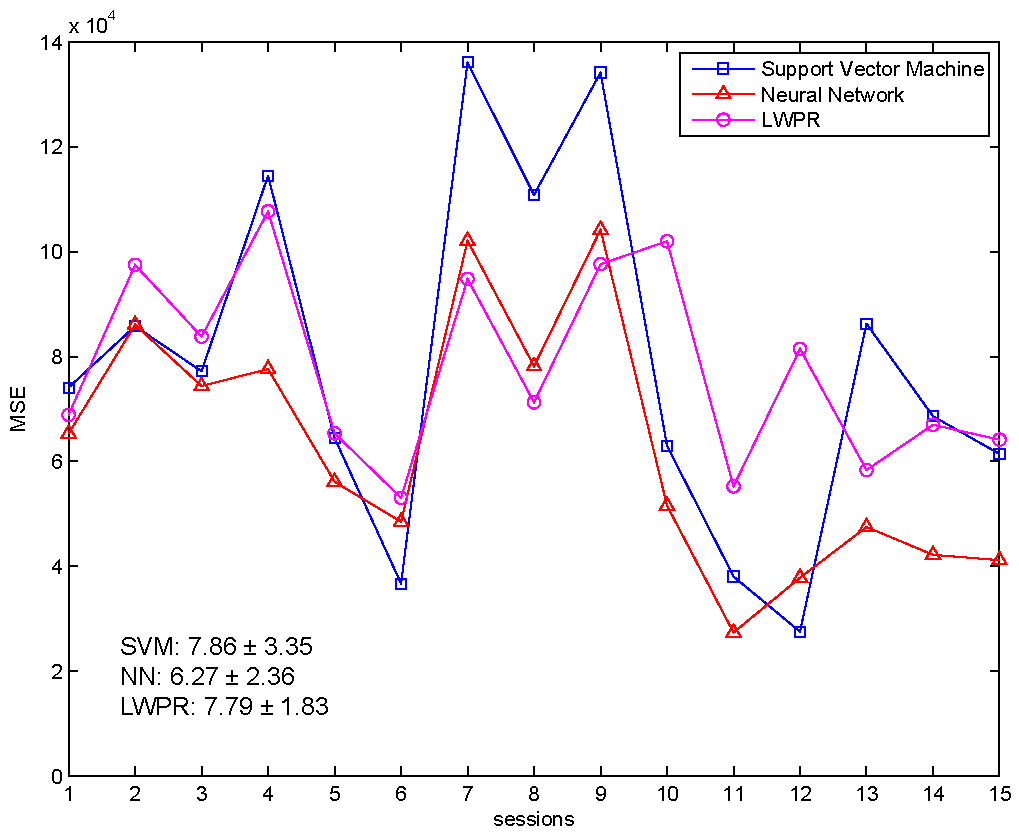
\includegraphics[width=0.4\textwidth]{figs/fig_MSE_regr_resCrossBestOnDay1} \\
    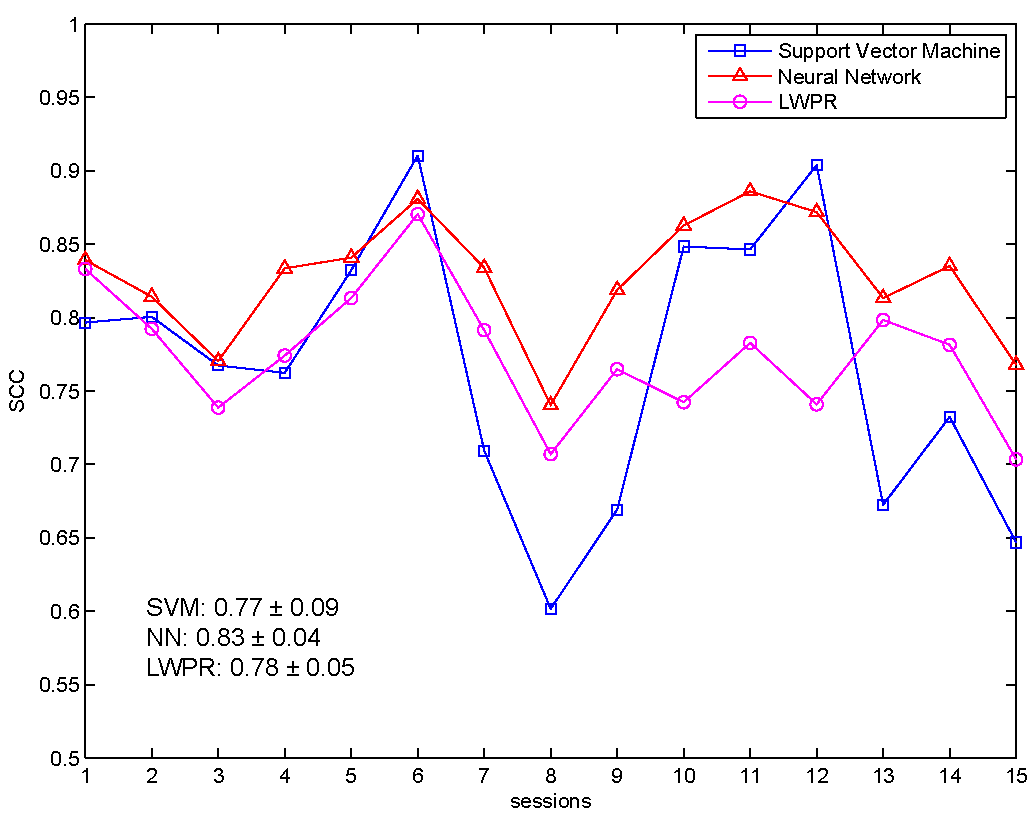
\includegraphics[width=0.4\textwidth]{figs/fig_SCC_regr_resCrossBestOnDay1} \\
  \end{tabular}
  \caption{Regression accuracy of best models, day $1$. Top to bottom:
    MSE, Normalised Root MSE, Squared Correlation Coefficient.}
  \label{fig:best_regr}
\end{figure}

Figure \ref{fig:best_regr} shows the results for day $1$. Consider the
first pane, plotting the NRMSE for each session: as it is apparent, as
it was for classification, there is no clear advantage of one approach
over another. NNs perform slightly better as far as the NRMSE is
concerned, which is probably the most interesting measure of
performance, when moving to a real setting. Their error is on average
$10.54\% \pm 1.41\%$ and $10.01\% \pm 1.93\%$. But as well, both LWPR
and SVM perform quite well, their average errors ranging from
$10.54\%$ to $11.98\%$.

Consider now the second and third panes of the Figure. First of all
there is a clear inverse correlation between the MSE and the SCC, as
it is expected: for both days and for all approaches, a larger MSE
corresponds to a lower SCC. Secondly, it is once again clear that the
generalisation performance strongly depends on which data we have used
to train the machines: consider for instance the MSE attained by SVM
on day $1$ (Figure
\ref{fig:best_regr}, second row): the best model was trained upon
data coming from sessions $6$ and $12$, although uniformised, and not
surprisingly those are the sessions for which the MSE is minimum; the
same effect is present for the other approaches.

Lastly, in practical terms: the best average MSE obtained by NNs
($6.27\cdot 10^4 \pm 2.36\cdot 10^4$ and $4.76\cdot 10^4 \pm 1.52\cdot
10^4$) corresponds to, in turn, an average error of 5N and
$4.36$N. Figure \ref{fig:regression} shows some samples of the force
values obtained from the OFTS, along with the corresponding values
predicted by the best approach, that is, NNs. As one can see, despite
the non perfect correspondence of the two curves, the NN definitely
follows the real target to a remarkable degree of accuracy, for a wide
range of frequencies of the pressing/releasing action.

\begin{figure}\centering
  \begin{tabular}{c}
    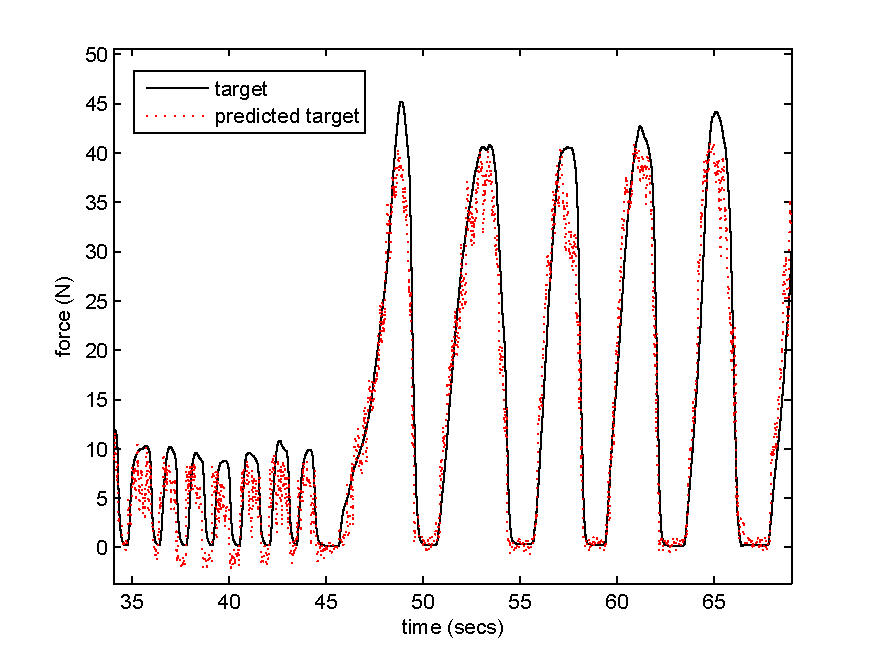
\includegraphics[width=0.45\textwidth]{figs/fig_regression1}\\
    \includegraphics[width=0.45\textwidth]{figs/fig_regression2}
  \end{tabular}
  \caption{Examples of the force target value, as guessed by our
    Neural Network. (upper pane) session $6$, day $1$, MSE: $4.85\cdot
    10^4$; (lower pane) session $10$, day $2$, MSE: $5.48\cdot 10^4$}
  \label{fig:regression}
\end{figure}
